\documentclass[10pt]{article}
\usepackage[utf8x]{inputenc}
\usepackage{amsmath, amsthm, amsbsy, rotating,float}
\usepackage{graphicx,algorithm,algorithmic,subfig}
\usepackage{setspace,enumerate}
\doublespacing




\author{Esteban D\'{i}az}
\title{Homework 1}{}

\begin{document}
\maketitle

\section{Plotting of given distributions}
\begin{figure}[H]
    \centering
    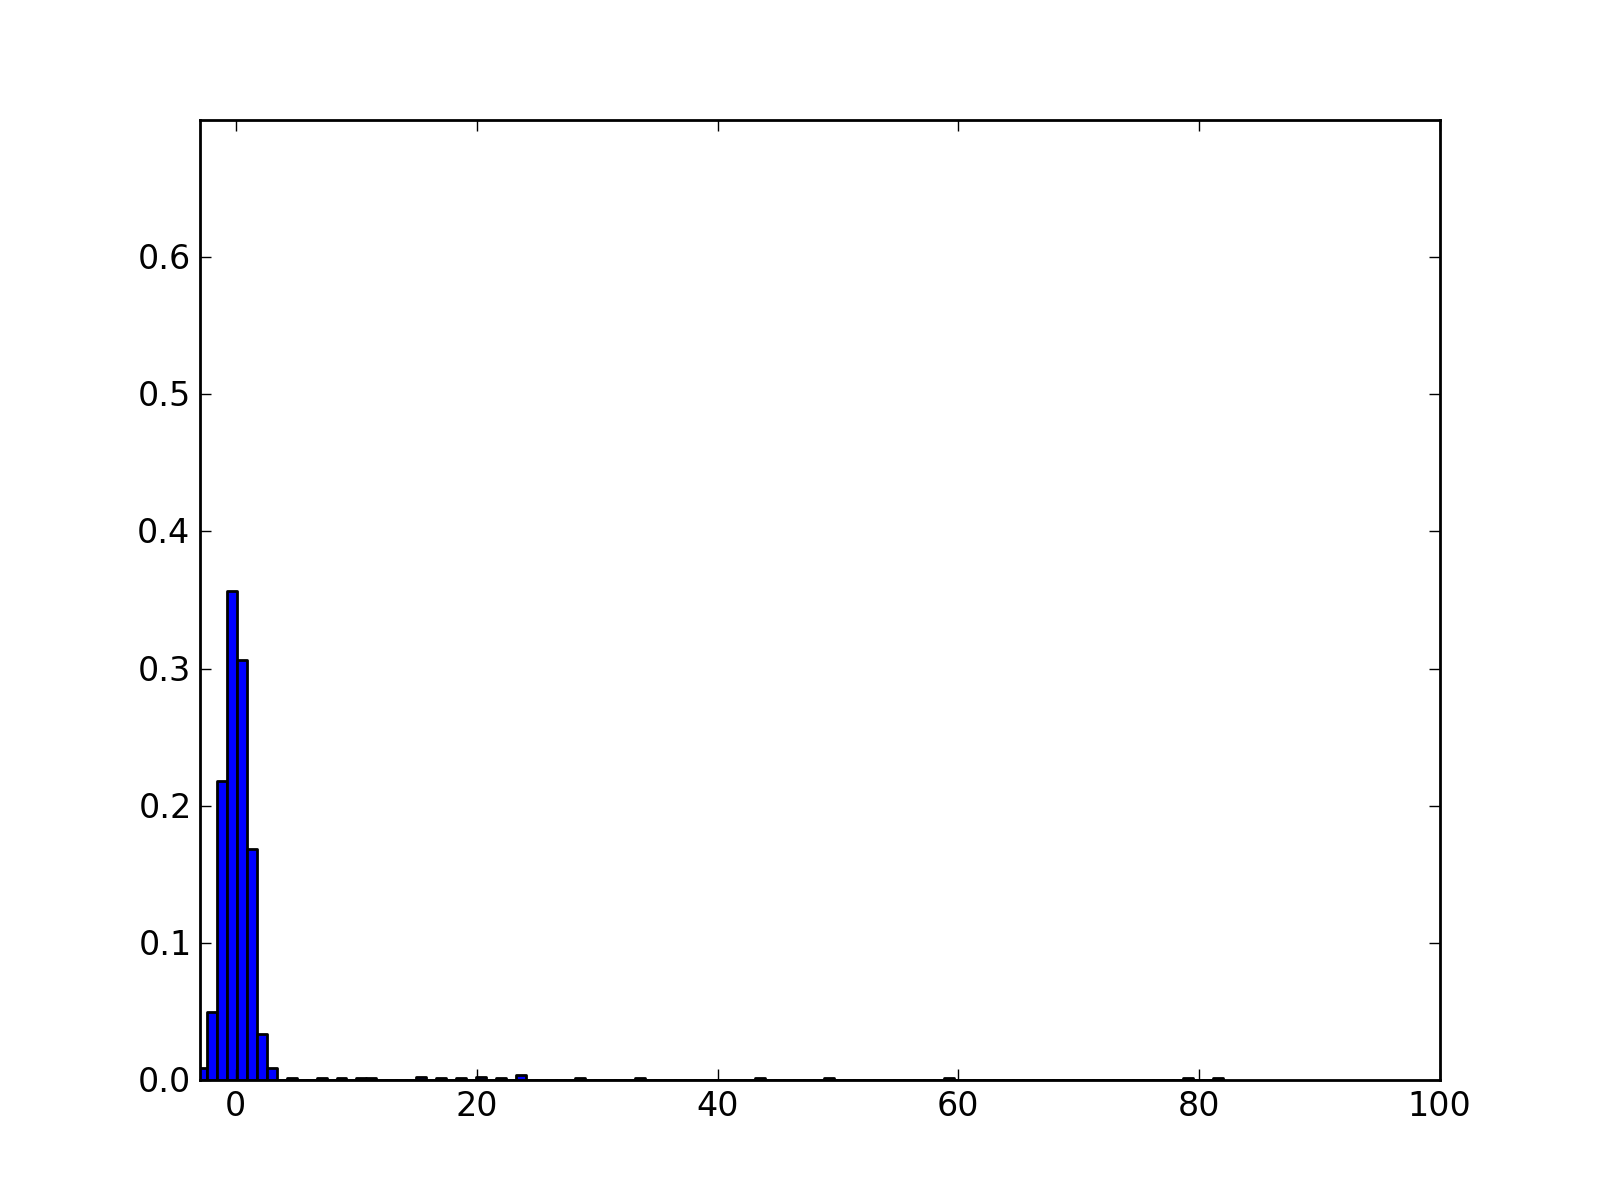
\includegraphics[width=0.85\textwidth]{../fig1.png}
    \caption{Gaussian mix: 95\% $N(0,1)$ and 5\% $N(0,36)$}
    \label{fig:fig1}
\end{figure}

\begin{figure}[H]
    \centering
    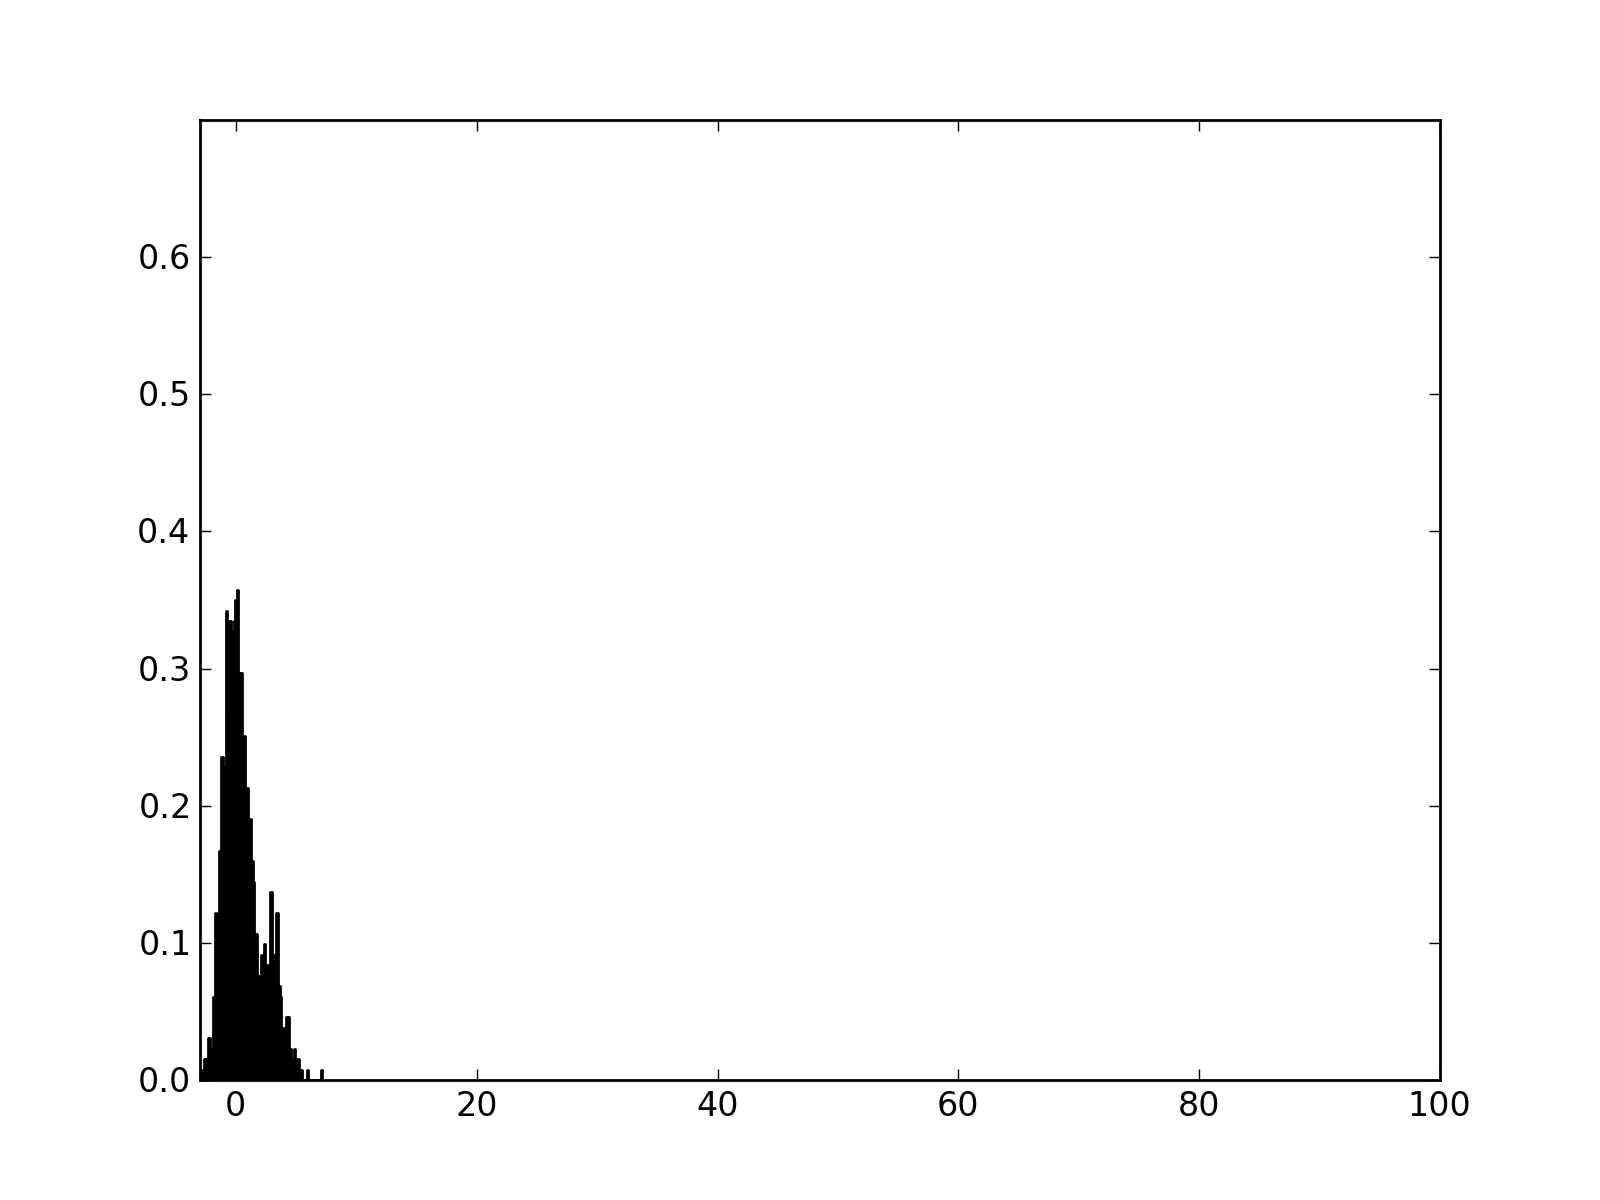
\includegraphics[width=0.85\textwidth]{../fig2.png}
    \caption{Gaussian mix: 80\% $N(0,1)$ and 20\% $N(3,1)$}
    \label{fig:fig2}
\end{figure}

\begin{figure}[H]
    \centering
    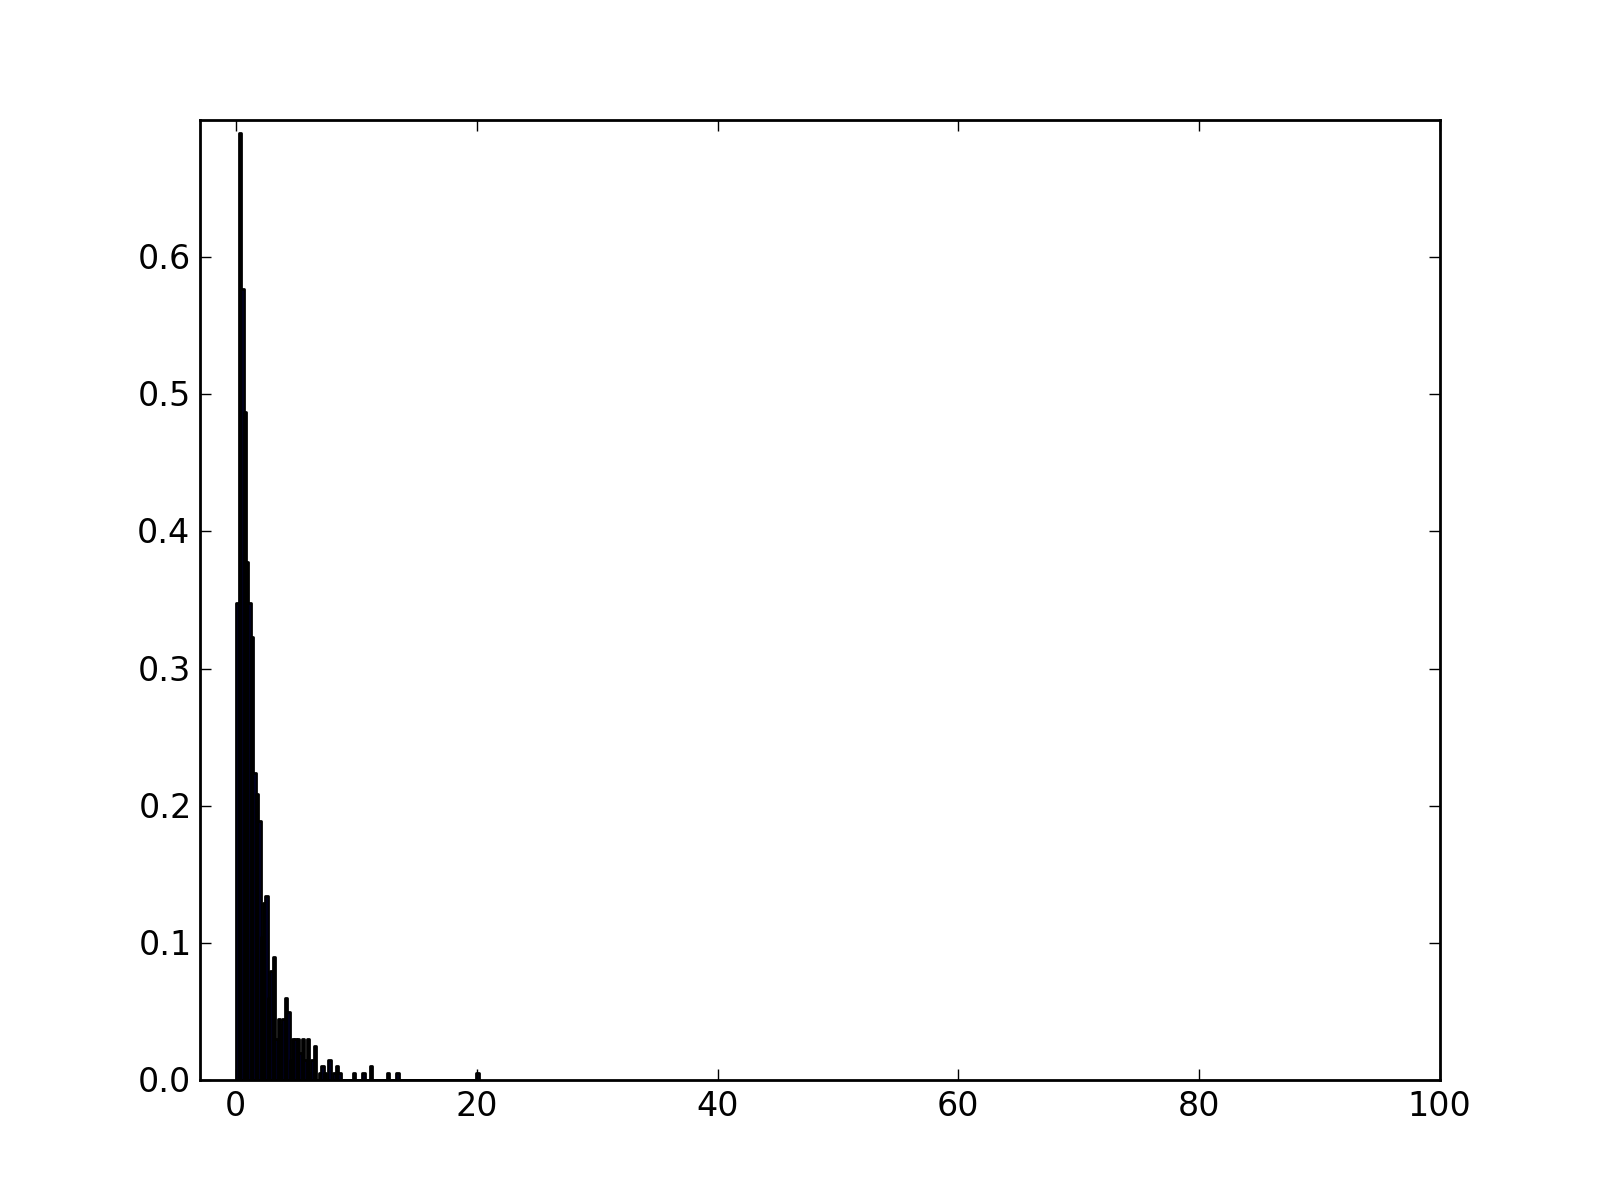
\includegraphics[width=0.85\textwidth]{../fig3.png}
    \caption{Log normal distribution: $LN(0,1)$}
    \label{fig:fig3}
\end{figure}

\section{Comparison between Gaussian distributions}
Let $X \sim N(\mu,3\sigma^2)$ and $Y \sim N(\mu,\sigma^2)$:
\begin{enumerate}
    \item $P[X \geq Y]=P[Y\geq X]$: this relation is false because
          $X$ is more spread around $\mu$ than $Y$, therefore, $P[X \geq Y]>P[Y\geq X]$.
    \item $P[X\geq \mu -1] = P[Y\geq \mu -1]$: false, given that $Y$ is more narrow than $X$
          then its integral is greater than  the one on $X$ since more values are to the left
          of $\mu -1$. 
    \item $P[X \leq \mu]=P[Y \geq \mu]$: this statement is true, and both probabilities are
          $P=0.5$. Both p.d.f. sum to 1, and are centered at $\mu$, so the integral to either
          side has to be 0.5 .
    \item $P[ \left|X-\mu \right| <\sigma]= P[\left|Y-\mu\right|<\sigma]$: this statement
          is false. $Y$ has a more narrow distribution than $X$, therefore 
          $P[\left|Y-\mu\right|<\sigma] > P[ \left|X-\mu \right|$.
    \item $P[ \left|X-\mu \right| <\sqrt{3}\sigma]= P[\left|Y-\mu\right|<\sigma]$: true. In 
          this case both probabilities describes the inter quartile range. 
\end{enumerate}


\section{Problem 2.29}
Two fair dice are rolled. Let $X$ be the probability of the absolute difference between
the outcome of the dice:
\begin{itemize}
    \item Find the p.m.f and the c.d.f. of X
    \item Find $P(0<X\leq 3)$ and $P(1\leq X <3)$
\end{itemize}

For the 36 combinations of the two fair dice we have 6 possible outcomes $X=0,1,2,3,4,5$.

For example, for $X=0$ we have 6 combinations (having the same outcome on both dice). 
For $X=1$ we have 10 ($|2-1|$,$|3-2|$,$|4-3|$,$|5-4|$,$|6-5|$)*2, and so on.

The c.d.f is defined as $P(X\leq x)=\sum_{k\leq x} f(k) $

\begin{tabular}{c |c | c }

   $X$    & p.m.f  & c.d.f \\ 
    0     & 6/36   & 6/36  \\ 
    1     & 10/36  & 26/36 \\
    2     & 8/36   & 24/36 \\ 
    3     & 6/36   & 30/36 \\
    4     & 4/36   & 34/36 \\
    5     & 2/36   & 1     \\
\end{tabular}

$P(0<X\leq 3) = 24/36$ and $P(1\leq X <3)18/36$


\section{Problem 2.33}
Analysis of a c.d.f.:

\begin{itemize}
    \item Is the r.v discrete or continuous? The way that the 
          graph is plotted shows that X is continuous with $X \in (0,3.5)$.
    \item What is the probability of $1\leq X \leq 3$? The probability is 
          $F(3)-F(1)= 0.4$ with $F(x)$ being the c.d.f.
    \item $P(X\geq1)=F(3.5)-F(1)=0.6$ 
\end{itemize}


\section{Problem 2.34}
\begin{itemize}
    \item Is the r.v discrete or continuous?  The r.v. is discrete
    because it takes a finite number of outcomes.
    \item $P(1\leq X<2)=0.8$
    \item $P(X\geq 1)=F(2)-F(1)=0.2$

\end{itemize}

\end{document}
